
\documentclass[a4paper,10pt]{article}
\usepackage{listings,color,epsfig,amsmath,url}
\definecolor{codecolor}{rgb}{0.99,0.97,0.94} % color values Red, Green, Blue
\definecolor{commentcolor}{rgb}{0.1,0.5,0.1} % color values Red, Green, Blue
\definecolor{stringcolor}{rgb}{0.3,0.1,0.1} % color values Red, Green, Blue
\newcommand{\Code}[1]{\texttt{#1} }
\newcommand{\code}[1]{\Code{#1} }
\newcommand{\DB}   {\code{{MOOSDB}}}
\newcommand{\MA}   {\code{{MOOSApp}}}
\newcommand{\Ignore}[1]   {}



% Title Page
\title{Logging with \code{pLogger}}
\author{Paul Newman}


\begin{document}
\maketitle

\begin{center}

\epsfig{file=images/moose6.eps,width = 0.2\linewidth}
\end{center}

\section{Logging -- \code{pLogger}}
The \code{pLogger} process is intended to record the activities of
a MOOS session. It can be configured to record a fraction of or
every publication of any number of MOOS variables. It is an
essential MOOS tool and is worth its weight in gold in terms of
post-mission analysis, data gathering and post-mission replay.

The configuration of \code{pLogger} is trivial and consists of
multiple lines with the following syntax:
\begin{center}
\code{Log} =  {\it{varname}} @ {\it{period}} $[NOSYNC],[MONITOR]$
\end{center}
where {\it{varname}} is any MOOS variable name and {\it{period}}
is the minimum interval between log entries that will be recorded
for the given variable. For example, if
{\it{varname}} = \code{INS\_YAW} and {\it{period}} = 0.2 then even
if the variable is published at 20Hz it will only be recorded at
5Hz. The optional \code{NOSYNC} flag indicates that this variable
should not be recorded in the synchronous logs (see Section
\ref{sec:LogTypes}). The optional \code{MONITOR} flag tells \code{pLogger} to send a notification if this variable isn't logged at least every 10 seconds. The notification occurs under the \code{MOOS\_DEBUG} variable. If you are running \code{iRemote} (which subscribes to this variable
automatically) you'll see a warning printed to the screen. This can be pretty useful when running
a complicated system and you really do want notification that an important variable isn't being logged (probably because the process producing the variable is kaput in some sense.)

\subsection{Logging Session}

The logger supports the notion of logging sessions. For each log session the logger will create a new directory and place all the logged files within that directory. These are typically (see later sections) an {\it{alog}} file, a {\it{slog}} file, a system log file, a copy of the mission file (moos file) and, if applicable, a hoof file (if  \code{pHelm} is running). A new log session can be created by writing the variable \code{LOGGER\_RESTART} to the \code{MOOSDB} or if you are using \code{iRemote} by pressing shift-g.

\subsection{Log File Types}\label{sec:LogTypes}
The logger records data in two file formats -- synchronous
(``slog'' extensions) and asynchronous (``alog'' extensions). Both
formats are ASCII text -- they can always be compressed later and
usability is more important than disk space. The two formats are
now discussed.

\subsubsection{Synchronous Log Files}
Synchronous logging makes a table of {\em{numerical}} data. Each
line in the file corresponds to a single time interval. Each
column of the table represents the broad evolution of a given
variable over time. The time between lines (and whether
synchronous logging is even required) is specified with the line:
\begin{center}
\code{SyncLog}= {\it{true/false @ period}}
\end{center}
where {\it{period}} is the interval time.

If there has been no change in the numeric variable between
successive time steps, then its value is written as \code{NaN}. It
is important to note that synchronous logs do not capture all that
happens -- they sample it. Synchronous logs are designed to be used
to swiftly appraise the behaviour of a MOOS community by examining
numeric data in a tool such as Matlab or a spreadsheet. The
\code{MOOSData} Matlab script reads in these files and with a
single mouse click can display the time evolution of any logged
variable.


\subsubsection{Asynchronous Log Files}
Asynchronous logging is thorough. The mechanism is designed to be
able to record {\em{every}} delta to the MOOSDB. The use of the
period variable allows the mission designer to back off from this
ultimate limit and record variables at a maximum frequency. The
key properties of asynchronous logging can be enumerated as follows.
\begin{enumerate}
\item Records both string and numeric data.
\item Records data in a list format -- one notification per line.
\item Entries are only made when variable is written.
\end{enumerate}
Asynchronous log files are designed to be used with a playback
tool (for example \code{uPlayback} or other purpose-built
executable). Although the handling of strings and numeric data
adds a slight overhead to such a program's complexity, the utility
gain from being able to slow, stop and accelerate time during a
post-mission replay/reprocessing session is simply massive. Turn asynchronous logging on with:
\begin{center}
\code{AsyncLog = true}
\end{center}
in the logger configuration block.

\subsubsection{Compressed Asynchronous Logging}
If the the common compression library Zlib is available\footnote{this might be a bit tricky on WIN32 platforms.}  pLogger offers the ability to compress alog files at run time. The CMake build system will search for the correct libraries and headers and set \code{ZLIB\_FOUND} if all is good at compile time. You can turn on compressed logging by adding

\begin{center}
\code{CompressAlogs = true}
\end{center}

to the configure block of \code{pLogger}\footnote{If you are in the habit of launching processes via \code{pAntler} and kill them all in one swoop by pressing ctrl-C in pAntlers window then take care...on Windows child processes are not killed by passing signals so \code{pLogger} has no chance to tidy up the compression routines. On Nix platforms Antler offers support for  killing child processes in a compassionate  way and so compressed log integrity is ensured.}

\subsection{System Log File}
There is a third kind of log file that is produced -- a system log file (ylog). This file only contains
data contained in \code{MOOS\_SYSTEM} and \code{MOOS\_DEBUG} messages. The later can be written to by calling the \code{CMOOSApp::MOOSDebugWrite} method from any \code{CMOOSApp} derived class. The thinking behind the ylog files is that it is pretty useful to be able to browse through
a text file of events to see when and if things went wrong in a mission. Processes can write to \code{MOOS\_SYSTEM} and/or \code{MOOS\_DEBUG} if something happens which they think is salient. Think of this as \code{/var/log}.


\subsection{Dynamic Logging Configuration}
Post V7.0.1 releases of MOOS include a dynamic logging ability. External parties can, at run time, request the logger to start logging
particular (named) variables. The logger subscribes to messages called \code{PLOGGER\_CMD} (if the Logger is being run under the MOOS name ``pLogger'', otherwise substitute the relevant name) and by correctly formatting the string data of this message dynamic logging can be invoked.

\begin{center}
\code{LOG\_REQUEST} =  {\it{varname}} @ {\it{period}} $[NOSYNC],[MONITOR]$
\end{center}

Note that this string format is identical to that found in the mission file, modulo \code{LOG} being replaced with \code{LOG\_REQUEST}. Now dynamic logging sits naturally with ``alog'' (asynchronous) files but not so well with ``slog'' files. These files are easy to use (and hence popular)  because they are rectangular numerical arrays written to text file (easily parsed by Matlab's load command). But dynamic logging means that by the time a mission ends an unknown number of variables (columns) will occur in every line of the slog. To address this issue the logger can be configured (in its mission file configuration block) with a line like:

\begin{center}
\code{DynamicSyncLogColumns} =  30
\end{center}

Here 30 columns are being reserved for variables that are requested at run time. As dynamic requests are received and processed by the logger, these unclaimed columns are consumed until none remain. At this point any future dynamic logging requests will still be accepted but the logged variables won't appear in the slog file (they will of course appear in the {/it{alog}} file). Unclaimed slots will be labeled \code{DYNAMIC\_X} until claimed and will always have \code{NaN} entries.

\subsection{Specifying Log File Names and Locations}\label{Sec:Places}

Each time the logger starts it creates (if required) a new directory in the logging root directory (see below) and performs logging within that directory. \code{pLogger} is quite flexible in terms of log file configuration and is controlled by the following variables.

\begin{description}
\item{\code{GlobalLogPath}} This is a {\textbf{file scope variable}} (i.e. not in any process configuration block). If it is present in a mission file, then it specifies the root directory in which log files will be created.
\item{\code{Path}} This specifies the root logging directory but is only used if \code{GlobalLogPath} is not set (see above).
\item{\code{File}} This is the stem file name given to logged files (alog/slog and ylog).
\item{\code{FileTimeStamp}} If this is set to true, the name of  each logged file (and created containing directory) will be the concatenation of the \code{File} variable and a time stamp. If \code{FileTimeStamp} is false then each time the logger is run it will write to the same set of log files {\textbf{and destroy the original contents}}. This is by design; when developing, it's often useful to not have useless log files take ever more space on your machine.
\end{description}

Note that if the logger is run without a mission file it starts logging to the local directory with file time stamping enabled. See Figure \ref{fig:LoggerConfig} for a typical logger configuration block.

If for some reason the logger was unable to start logging to a location specified in the log file it tries, as a last resort, to open a log directory in the current working directory (`.'). If this fall-back fails then all is lost, we are without hope and the logger exits. If you are running a mission from \code{pAntler}, you'll be notified that the logger has quit.


\subsubsection{Where is the Most Recent Log File?}


\code{pLogger} records where it last opened a log file in a file which by default is called ``. LastOpenedMOOSLogDirectory" (note the period !) and is in the working directory of the logger. The location and name of this hint file can be customised via the \code{LoggingDirectorySummaryFile} parameter, for example

\begin{center}
\code{LoggingDirectorySummaryFile} =  /homes/5/spock/.MOOSLoggingHint
\end{center}.

Why is this useful ? Well you can now quickly knock up a script which peeks in this hint file and opens for browsing the last set of log files.




\subsection{Mission Backup}
Simply having the {\it{alog}} and {\it{slog}} files is not enough
to evaluate the mission. One also needs the things that
{\em{caused}} the data to be recorded, namely the *.moos Mission
file and the *.hoof file (if Task redirection was used). To this
end the \code{pLogger} process takes a copy of these files and
places them (name appended with a time stamp if desired) within
the logging directory. The files extensions are renamed to
{\it{*.\_moos}} and {\it{*.\_hoof}} respectively.

\subsubsection{Additional File Backup on Demand}
It is quite within the bounds of reason that a system using MOOS makes use of
configuration (especially other files) which has content which should not reside inside a *.moos or *.hoof file.
\code{pLogger} provides a mechanism to back these files up on request at run time. Post V7.0.1, by writing to the \code{PLOGGER\_CMD}
variable any MOOS process can instruct the logger to back a local file up and place a copy in the current logging directory. See Section \ref{Sec:Places}. As always, the process \code{\_CMD} message is a string and for dynamic file back up should be formatted as:

\begin{center}
\code{COPY\_FILE\_REQUEST} =  \textit{PathToFile}
\end{center}

For example,

\begin{center}
\code{COPY\_FILE\_REQUEST} =  /home/VehicleQ/CameraCalibration.txt
\end{center}

would log `` /home/VehicleQ/CameraCalibration.txt'' to a file called ``CameraCalibration.\_txt'' in the current logging directory. Note the additional underscore which is in keeping with the backup style used for mission files. If the file being backed up has no extension, a ``.\_bak'' is added.

\subsection{Wildcard Logging}

Post V7.0.1 a new configuration option has been introduced which instructs the logger to log every change made to the MOOSDB to an {/it{alog}} file. \footnote{It does this by using a specialised MOOS IPC call to the DB which is not intended for daily use.} By writing

\begin{center}
\code{WildCardLogging} =  true
\end{center}

asynchronous logging will be turned on (even if \code{AsyncLog = false} is present in the configuration block) and every change to every variable will be logged to the current {/it{alog}} file. Some points to note:

\begin{itemize}
\item Wildcard logging only causes variables to be written to the current {/it{alog}} file. Synchronous logging is not affected.
\item If the log rates for variables have already been been specified at configuration then it is these rates that are used.
\item If wildcard logging is enabled, when the logger spots that variables that are not already known to it are being written to the DB it registers to be told about every change made (like \code{Log = XXX @ 0}).
\item By default wildcard logging is disabled. It was designed to be a safety net for situations in which many new variables are being created by a software team in a dynamic environment.
\item It may take up to a second for the logger to detect and subscribe for new MOOS variables. If new data is written multiple times before subscription can complete (i.e. within a second), the logger will be unable to capture these writes.
\end{itemize}


\subsubsection{Wildcard Logging Patterns}

If all you do is set \code{WildCardLogging} to be true then everything will be logged. There is every chance though that you may want finer control by specifying template patterns for variables you want logged and equally, variables you don't want logged. Two optional configuration parameters \code{WildCardPattern} and \code{WildCardOmitPattern} achieve this. Each takes a value of a comma separated list of  ``globbing'' expressions; each expression containing any character apart from a comma. Only ``*'' and ``?'' wildcards are supported.  For example

\begin{center}
\code{WildCardPattern} =  DB\_*, *\_LA?
\end{center}

will only log variables with names that begin ``DB\_'' or end in ``\_LA'' followed by a single character. By specifying patterns which should not be logged finer control can be gained

\begin{center}
\code{WildCardPattern} =  DB\_*, *\_LA? \\
\code{WildCardOmitPattern} =  *ME,X*
\end{center}

will only log variables with names that  begin ``DB\_'' or end in ``\_LA'' followed by a single character but do not end with ``ME'' or begin with an ``X''. You can specify these patterns individually or  in tandem, i.e. you can use \code{WildCardOmitPattern}  without \code{WildCardPattern}  and vice versa.

You can also have multiple instances of these pattern declarations:

\begin{center}
\code{WildCardPattern} =  DB\_*\\
\code{WildCardPattern} =  *\_LA? \\
\code{WildCardOmitPattern} =  *ME\\
\code{WildCardOmitPattern} = X*
\end{center}



\subsubsection{Exclusion Logs - ''xlogs''}

Not recording the right thing can be expensive so \code{pLogger} can provide a safety net for you by logging variables which either

\begin{itemize}
\item failed to match any  \code{WildCardPattern} patterns
\item matched a \code{WildCardOmitPattern}
\end{itemize}

to a so called "exclusion log" or \code{xlog}. By setting \code{WildcardExclusionLog=true} in the configuration block any thing sent by any MOOS process that would usually not appear in the \code{alog} will be captured in the \code{xlog}. The following truth table fully specifies the configuration and behaviour of exclusion logging. If a cell in the ''Omit'' column is true it means that a variable name matches a \code{WildCardOmitPattern} and similarly for the ''Accept" column.

\begin{center}
  \begin{tabular}{ |c|c|c|l| }
    \hline
    WildcardExclusionLog & Omit & Accept & Destination \\ 
    \hline
    false & false & true & not logged \\ 
    false & false & false & alog\\ 
    false & true & true& not logged\\ 
    false & true & false & not logged \\ 
    true & false & true & xlog\\ 
    true & false & false & alog \\ 
    true & true & true & xlog \\ 
    true & true & false & xlog\\ 
    \hline
  \end{tabular}
\end{center}





\subsection{Runtime File Backup}
In Post 7.0.1 releases, by writing a correctly formatted string value to the MOOS variable \code{PLOGGER\_CMD} processes within the MOOS community can request the logger to back up arbitrary files to the current log directory. For example, if the contents of a message with name \code{PLOGGER\_CMD} is set to
\begin{center}
\code{COPY\_FILE\_REQUEST = /home/pnewman/code/TheFile.xzy}
\end{center}
 and published to the \DB  it will result in a copy of `/home/pnewman/code/TheFile.xzy` being placed in the logging directory under the name `TheFile.\_xzy`- note the additional underscore. If the file in question has no extension then `.\_bak` is appended to the file name.


\subsection{Example Configuration}
\begin{figure}[ht!]
\begin{lstlisting}[]{}

//////////////////////////////////////////////
// Logger configuration block
ProcessConfig = pLogger
{
    //over loading basic params..lets be feisty
    AppTick  = 20.0
    CommsTick   = 20.0

    //all file names begin with this stem
    File        = SciPark29Mar

    //where is the root log directory
    PATH        = /home/doe/MOOSData/SciencePark/

    //yes we want some sync logging for crude
    //performance checking
    SyncLog     = true @ 0.2

    //yes we want async logging so we can replay
    // exactly what happened and record strings
    AsyncLog    = true

    WildCardLogging = false

    //yes append each created directory log file
    //with a time stamp DAY MONTH YEAR TIME
    FileTimeStamp   = true

    //what do we want to log
    //(zero means capture everything)
    Log     = LMS_LASER_2D @ 0 MONITOR
    Log     = LMS_LASER_3D @ 0 MONITOR
    Log     = MARGE_ODOMETRY @ 0
    Log     = DESIRED_RUDDER @ 0
    Log     = DESIRED_THRUST @ 0
    Log     = CAMERA_GRAB @ 0
    Log     = GPSData @ 0.4

}

\end{lstlisting}
\caption{A Typical \code{pLogger} configuration block}
\label{fig:LoggerConfig}
\end{figure}

\newpage

\section{Replay -- \code{uPB}}
There is a FLTK-based, cross-platform GUI application that can
load in {\it{alog}} files and replay them into a MOOS community as
though the originators of the data were really running and issuing
notifications. A typical use of this application is to ``fake''
the presence of sensor processes when reprocessing sensor data and
tuning navigation filters. Alternatively, it can be used in pure
replay mode, perhaps to render a movie of the recorded mission. The
GUI allows the selection of which processes are ``faked''. Only
data recorded from those applications will be replayed from the
log files.  There is a single class that encapsulates all the
replay functionality -- \code{CMOOSPlayback}. The GUI simply hooks
into the methods exported by this class. The GUI is almost self
documenting -- start it up and hold the mouse over various buttons.

\begin{figure}
\center 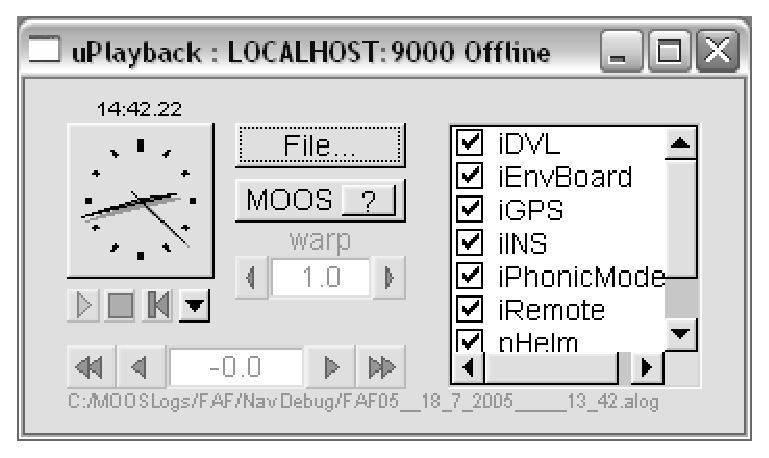
\epsfig{file=images/uPB.eps,width = 0.8\linewidth} \caption{A
screen shot of \code{uPB} -- a cross-platform ``alog'' playback
tool}
\end{figure}

A client process can control the replay of MOOS messages by
writing to the \code{PLAYBACK\_CHOKE} variable and writing a valid
time in the numeric message field. The Playback executable will
not play more than a few seconds past this value before waiting
for a new value to be written. In this way  it is possible to
debug (halt inspect and compile-in-place etc) at source level a
client application using replayed data without having the playback
rush on ahead during periods of thought or code-stepping.

\end{document} 